\begin{landscape}
\section{Data Description}
\begin{center}
\begin{longtable}{l | p{5cm} | p{1.5cm} | p{10cm}}
\label{tab:data}
No & Data Source &	Data Origin	& Description \\
\hline
1 &	F1 data, 2 csv files	& provided & \\
2 &	F2 data,  5 csv files	& provided &	49092 rows, 0-211 cycles, 44 var, Initial fermentation data \\
3 & F4 data, 7 csv files	& provided &	49092 rows, 0-213 cycles, 60 var, yeast product data \\
4 &	F5 data, 6 csv files	& provided &	49093 rows, 0-282 cycles, 52 var, Commercial yeast product data \\
5 &	F7 data, 6 csv files	& provided &	49092 rows, 0-225 cycles, 52 variables \\
6 &	F8 data, 6 csv files	& provided &	49092 rows, 0-135 cycles, 52 variables\\
7 & CSep data, 3 csv files	&provided \\	
8 &	MO data, 17 csv files	&provided \\	
9 &	Seps data, 9 csv files	&provided \\	
10&	SR data, 11 csv files	&provided \\
11&	Manual fermentation recordings,  
F2-F4 10 pdf, F5 2 pdf files&	provided&	processes manually filled in pdf. Data contains only F4 and F5 fermentations recordings  \\
12&	Brown colonies ferms, word doc
(Quality control results for few F4 and F5 batches)	&provided&	Data has attributes
\begin{itemize}
    \item Production Date (MM-DD-YYYY) -finished product date
    \item Strain (yeast strain no 7442 only)
    \item Seed - batch number
    \item Commercial – if F5
    \item Lot no - number of batches
    \item 	Status - quality control decision: Rejected, Released, Restricted release)
\end{itemize} \\
13&	Data Parameters - Excel with fermentation variable details  	&provided&Glossary, some variables description. Mainly variables represent a specified volume or mass of ingredients from yeast manufacturing formulas, also process condition measurements, such as an air or water temperatures, etc.\\

14&	Labelled Dataset - samples with statuses 
\begin{itemize}
    \item F2 samples: 1469 obs. of 45 variables
    \item F4 samples: 1252 obs. of 62 variables
    \item F5 samples: 294 obs. of 54 variables
\end{itemize}
&created& 	
Based on provided manual notes and quality control results.  
For few F2, F4 and F5 data there were manually assigned labels (statuses): \begin{itemize}
    \item REJECT
    \item RELEASE
    \item RESTRICT
\end{itemize}
\\
\hline
\end{longtable}
\end{center}
\end{landscape}

\section{Correlation plots of the parametric data}

\begin{figure}[ht]
    \centering
    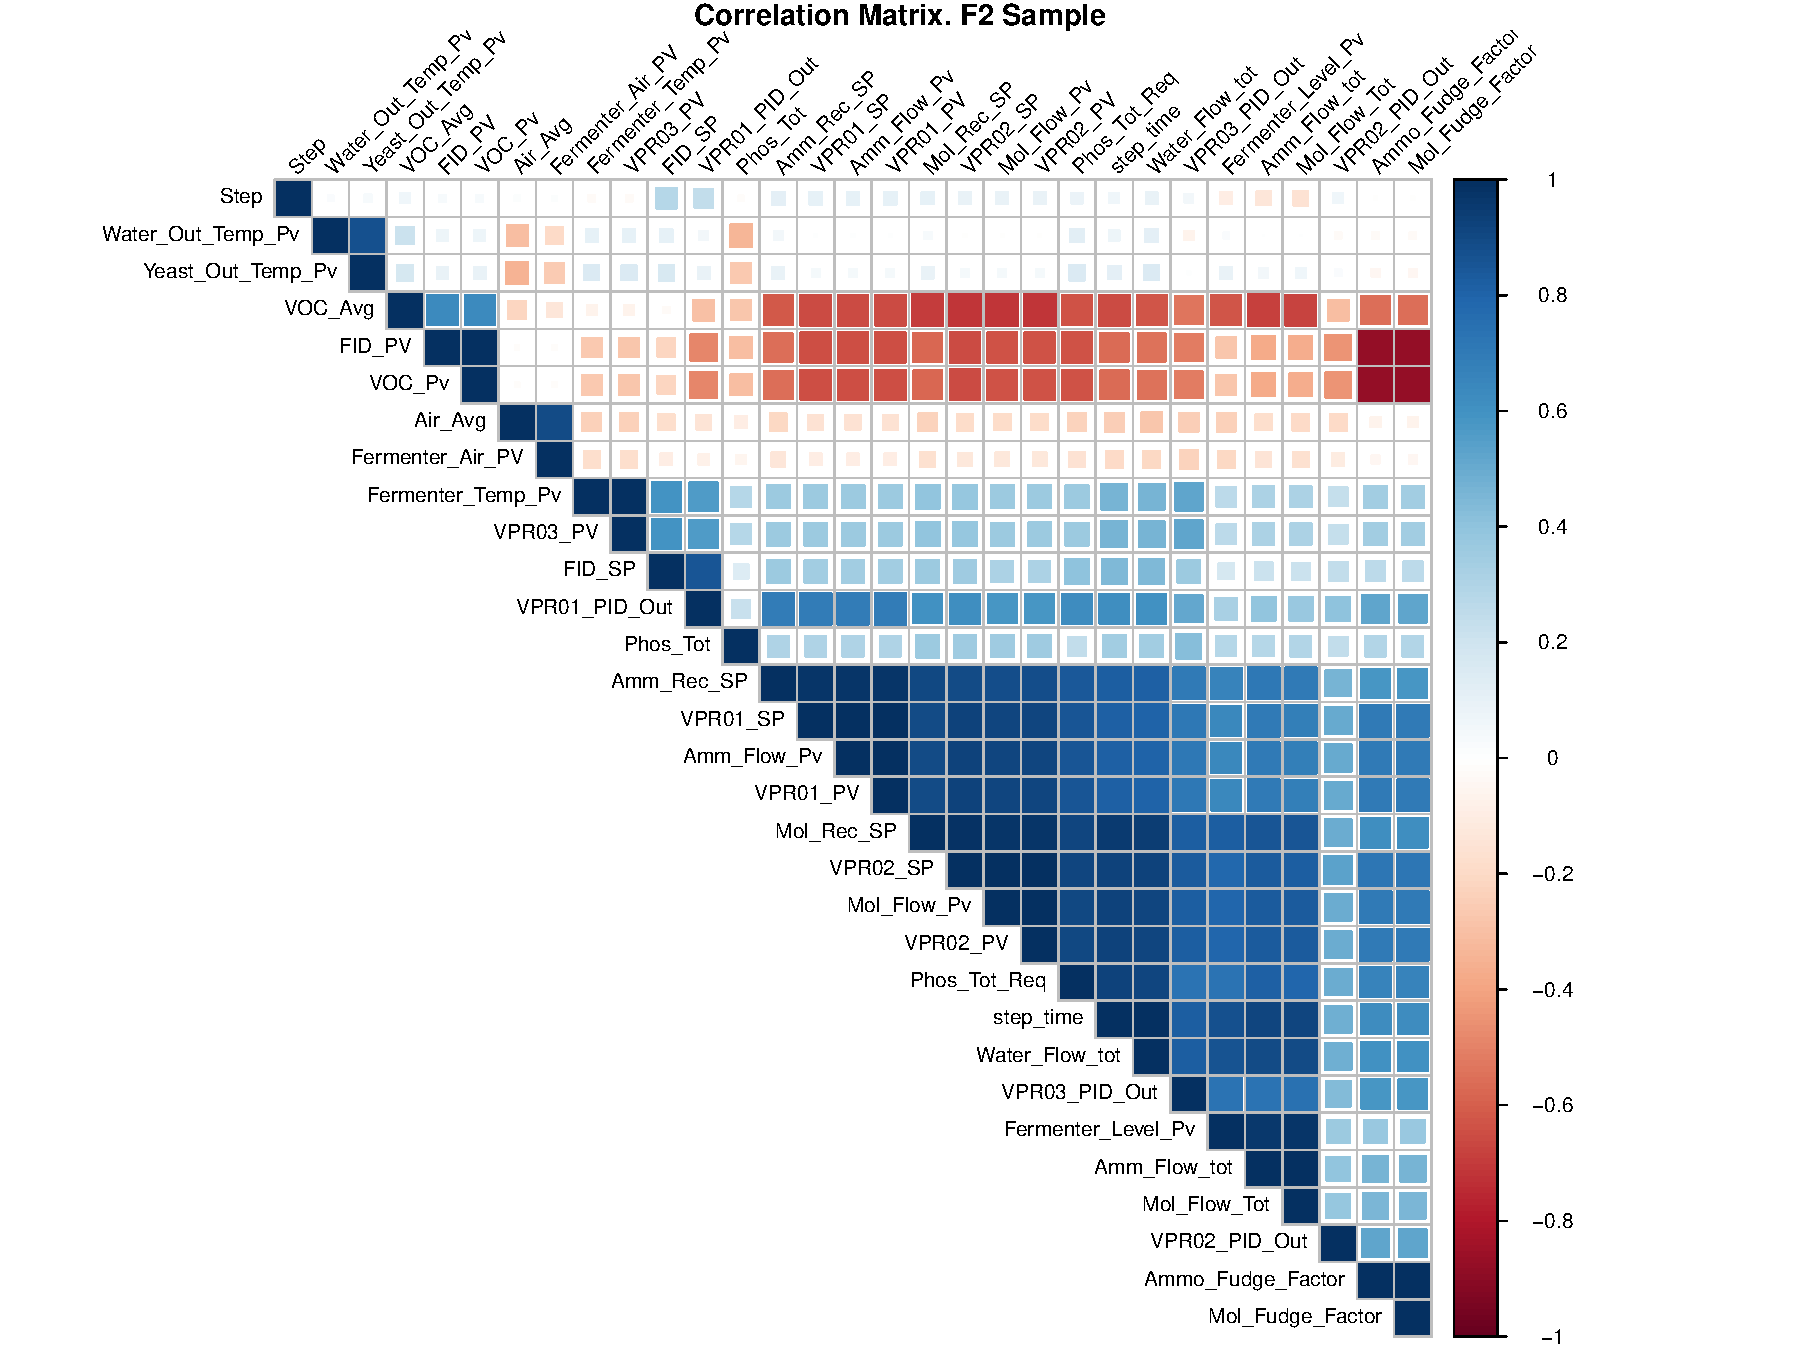
\includegraphics[width=1\textwidth]{plots/f2_correlation.pdf}
    \caption{F2 correlation matrix}
    \label{fig:f2_correlation}
\end{figure}

\begin{figure}[ht]
    \centering
    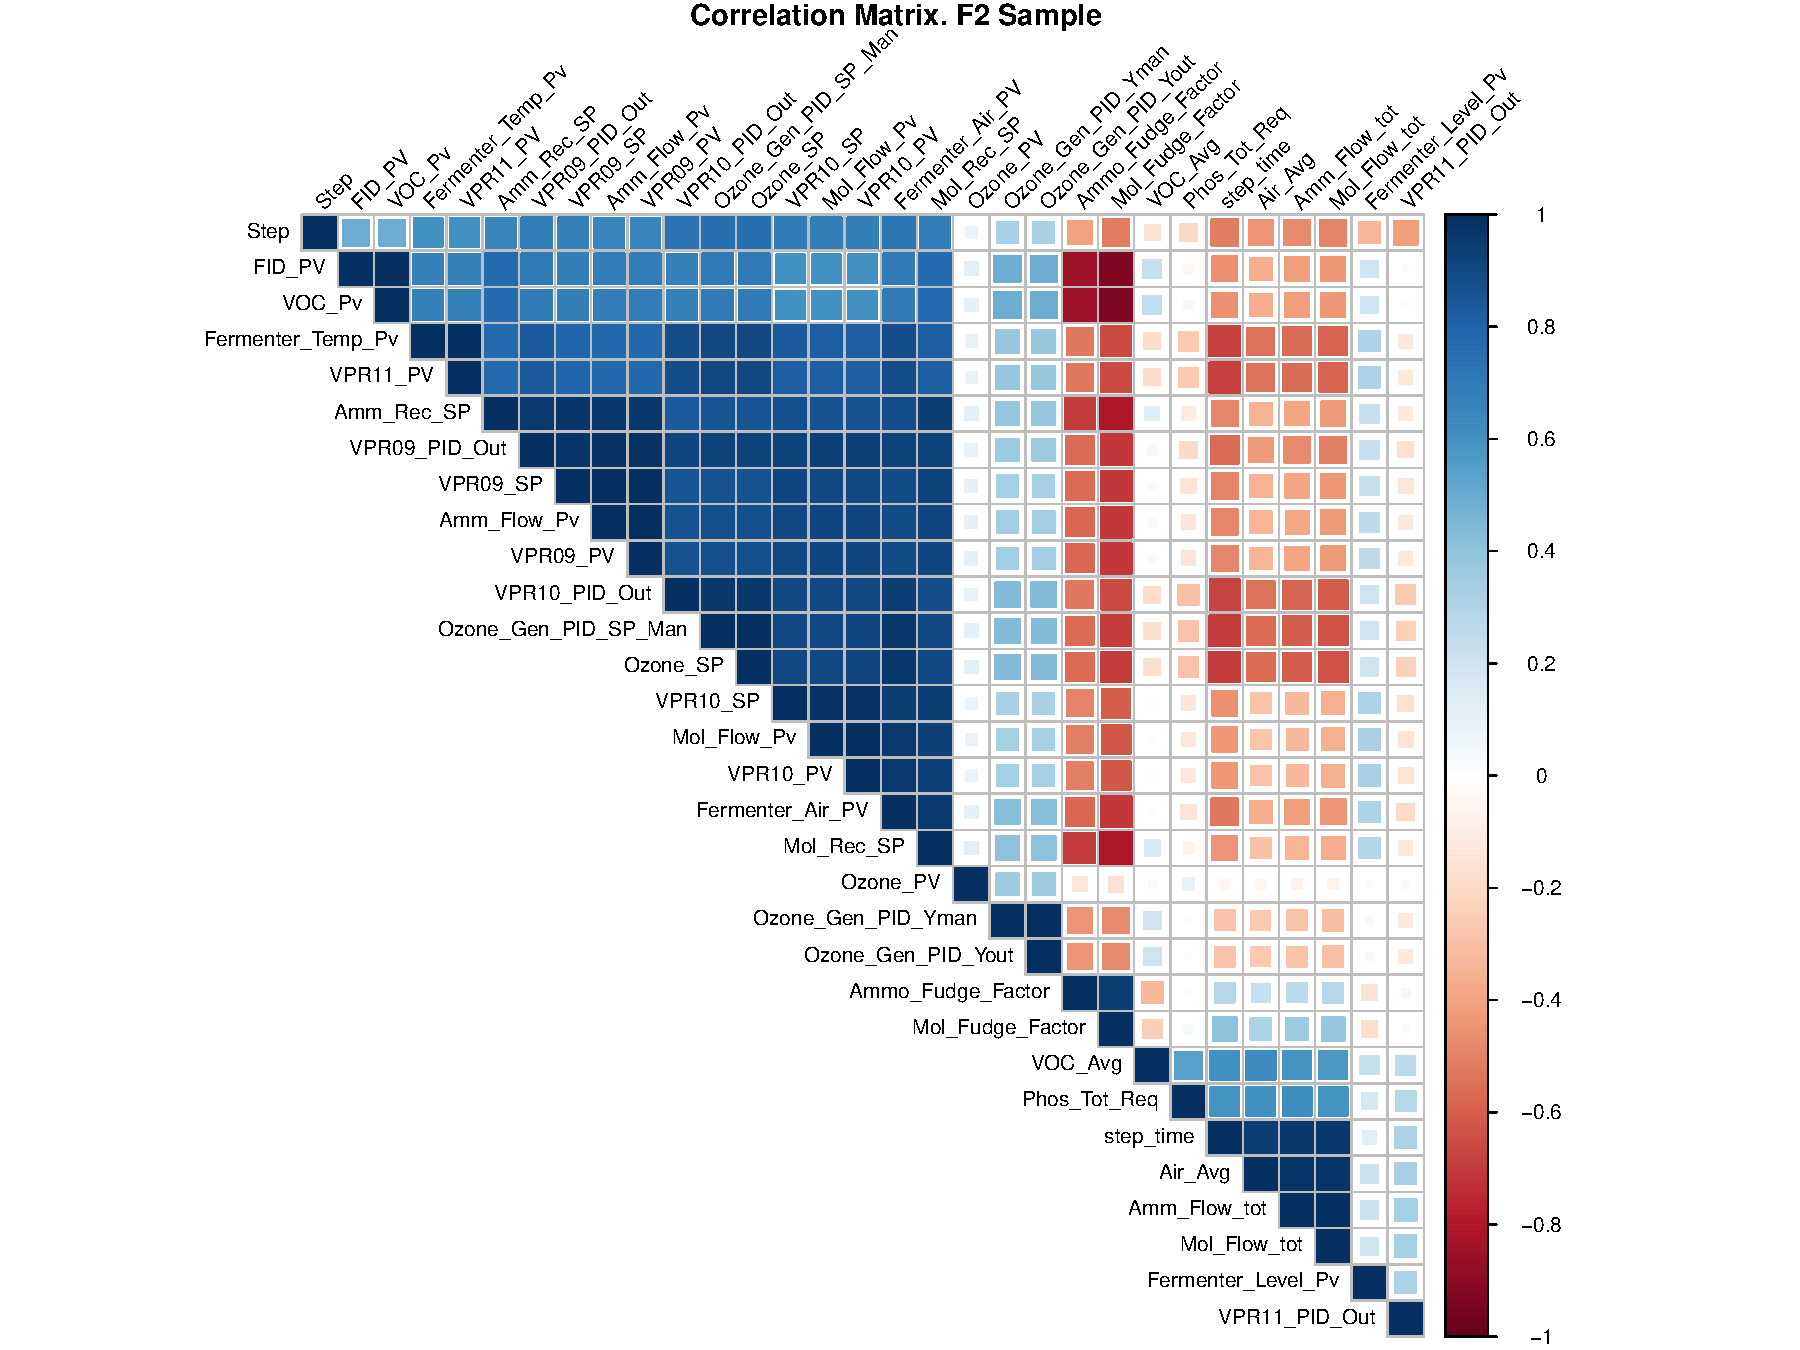
\includegraphics[width=1\textwidth]{plots/f4_correlation.pdf}
    \caption{F4 correlation matrix}
    \label{fig:f4_correlation}
\end{figure}

\begin{figure}[ht]
    \centering
    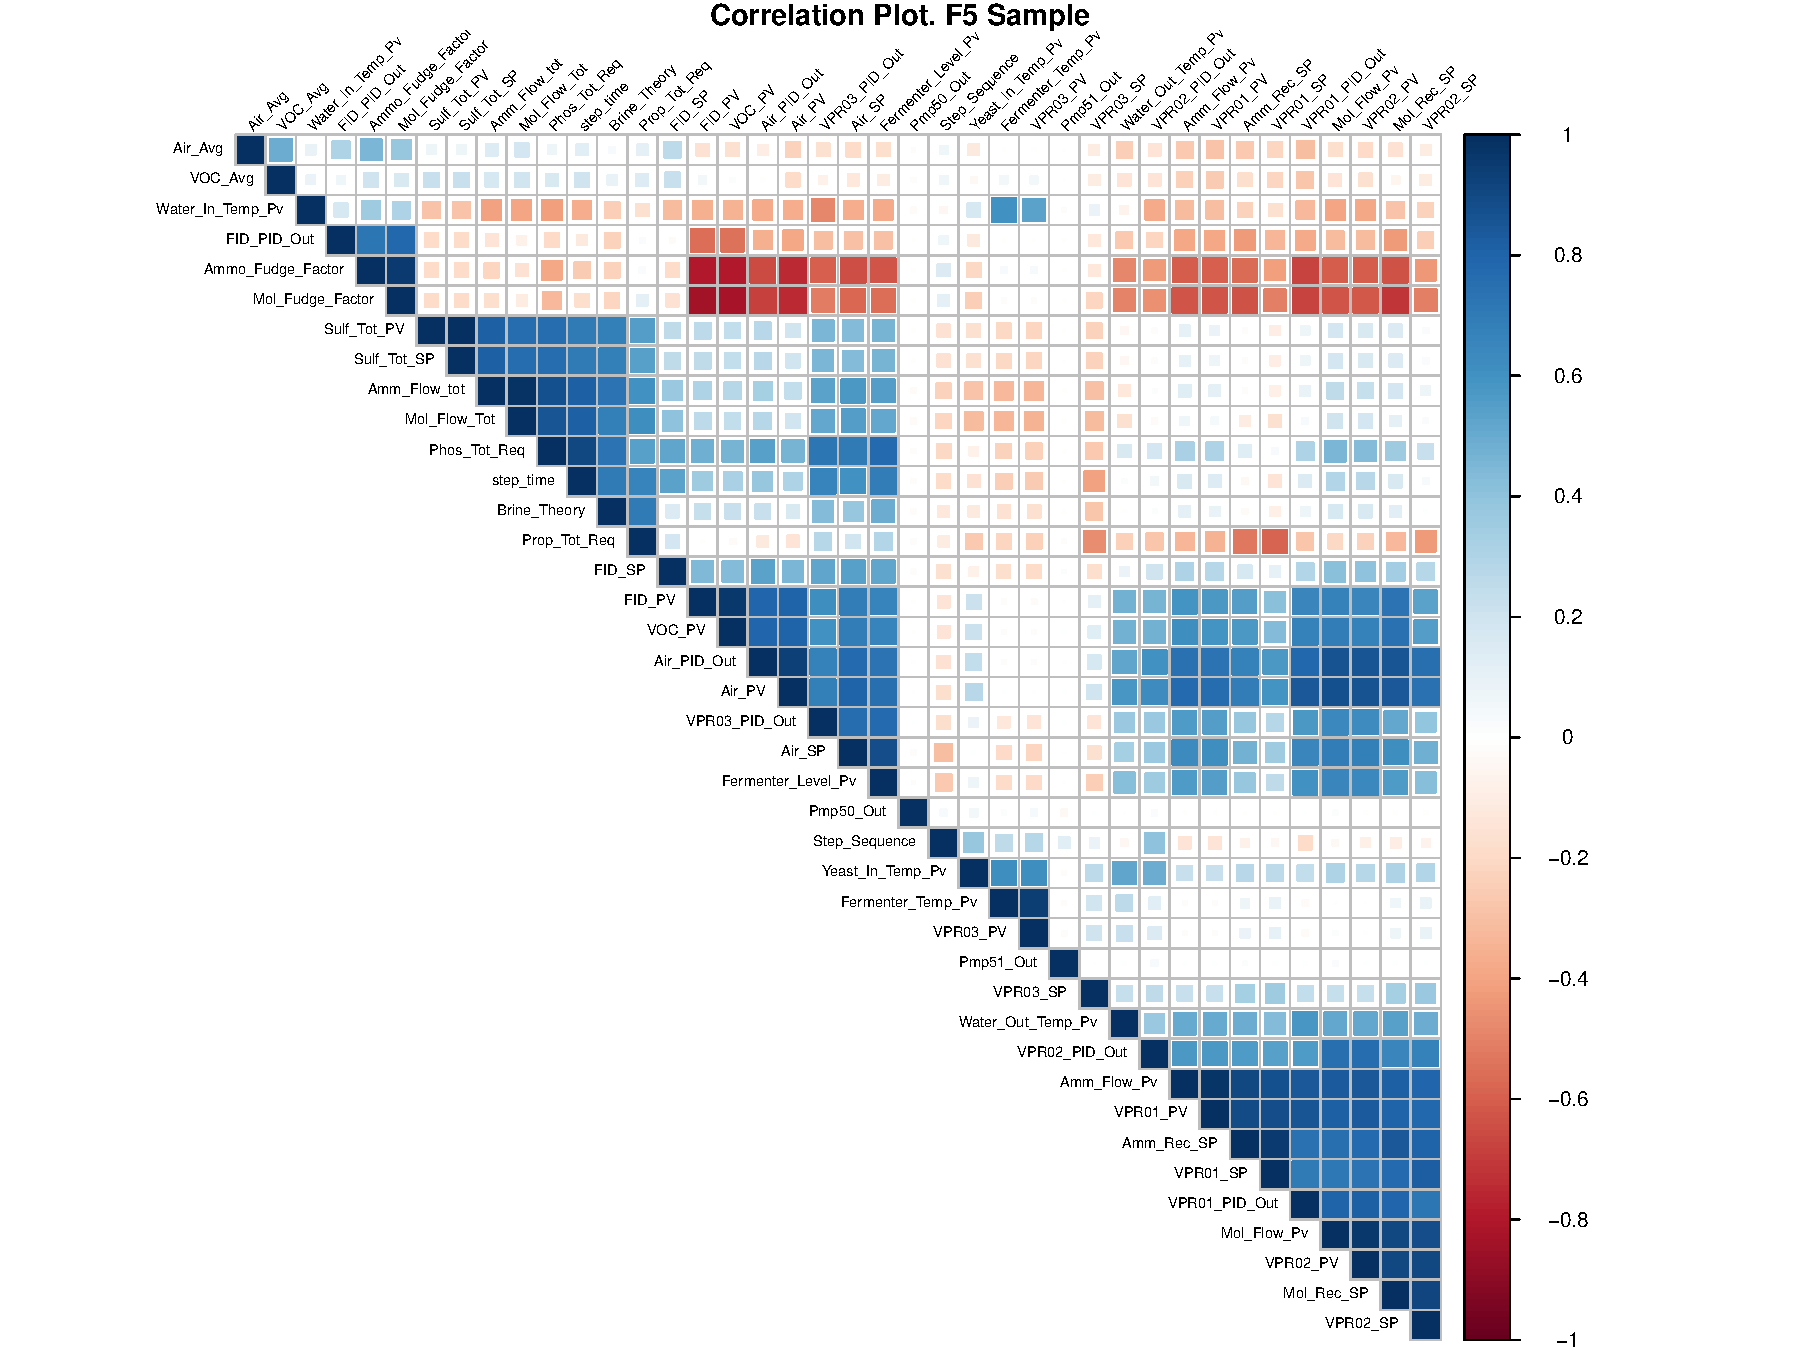
\includegraphics[width=1\textwidth]{plots/f5_sample_correlation.pdf}
    \caption{F5 correlation matrix}
    \label{fig:f5_correlation}
\end{figure}

\clearpage

\section{Summary description of the data}
\begin{table}[!htbp] 
\centering 
\resizebox{\textwidth}{!}{
\begin{tabular}{@{\extracolsep{5pt}}lccccccc} 
\\[-1.8ex]\hline 
\hline \\[-1.8ex] 
Statistic & \multicolumn{1}{c}{N} & \multicolumn{1}{c}{Mean} & \multicolumn{1}{c}{St. Dev.} & \multicolumn{1}{c}{Min} & \multicolumn{1}{c}{Pctl(25)} & \multicolumn{1}{c}{Pctl(75)} & \multicolumn{1}{c}{Max} \\ 
\hline \\[-1.8ex] 
F2\_Air\_Avg & 47,852 & 43.674 & 1.945 & 4.943 & 42.312 & 44.976 & 49.654 \\ 
F2\_Ammo\_Fudge\_Factor & 47,956 & $-$0.010 & 0.123 & $-$0.200 & $-$0.077 & 0.108 & 0.150 \\ 
F2\_Amm\_Flow\_Pv & 47,956 & 0.190 & 0.255 & 0.000 & 0.000 & 0.368 & 1.200 \\ 
F2\_Amm\_Flow\_tot & 47,956 & 114.688 & 150.950 & 0.000 & 0.000 & 203.098 & 652.059 \\ 
F2\_Amm\_Rec\_SP & 47,954 & 0.163 & 0.214 & 0.000 & 0.000 & 0.296 & 0.695 \\ 
F2\_Fermenter\_Air\_PV & 47,957 & 28.979 & 20.489 & 0.000 & 0.000 & 44.000 & 88.000 \\ 
F2\_Fermenter\_Level\_Pv & 47,956 & 2.511 & 1.591 & 0.000 & 0.834 & 3.697 & 5.445 \\ 
F2\_Fermenter\_pH\_Pv & 47,956 & 0.000 & 0.000 & 0.000 & 0.000 & 0.000 & 0.000 \\ 
F2\_Fermenter\_Temp\_Pv & 47,957 & 31.462 & 14.185 & $-$20.000 & 26.590 & 32.070 & 100.702 \\ 
F2\_FID\_PID\_Out & 21,349 & 0.000 & 0.000 & 0.000 & 0.000 & 0.000 & 0.000 \\ 
F2\_FID\_PV & 47,956 & 89.995 & 106.508 & 0.000 & 0.000 & 158.608 & 1,000.000 \\ 
F2\_FID\_SP & 47,956 & 126.187 & 24.608 & 100.000 & 100.000 & 150.000 & 150.000 \\ 
F2\_HMI\_Popup\_Sel & 4,032 & 0.200 & 0.000 & 0.200 & 0.200 & 0.200 & 0.200 \\ 
F2\_Mol\_Flow\_Pv & 47,956 & 3.065 & 3.768 & 0.000 & 0.000 & 6.403 & 18.927 \\ 
F2\_Mol\_Flow\_Tot & 47,956 & 1,710.765 & 2,276.169 & 0.000 & 0.000 & 3,045.860 & 8,462.040 \\ 
F2\_Mol\_Fudge\_Factor & 47,956 & $-$0.010 & 0.123 & $-$0.200 & $-$0.077 & 0.108 & 0.150 \\ 
F2\_Mol\_Rec\_SP & 47,956 & 3.161 & 3.353 & 0.000 & 0.496 & 5.581 & 15.000 \\ 
F2\_Phos\_Tot & 47,958 & 46.750 & 28.533 & $-$112.346 & 28.469 & 69.345 & 106.142 \\ 
F2\_Phos\_Tot\_Req & 47,956 & 7.971 & 9.476 & 0.000 & 0.000 & 17.800 & 39.000 \\ 
F2\_Step & 47,956 & 5.205 & 4.862 & 0.000 & 0.100 & 6.000 & 31.100 \\ 
F2\_step\_time & 49,092 & 325.628 & 395.488 & 0.000 & 0.000 & 645.792 & 1,384.916 \\ 
F2\_Sulf\_Tot\_pv & 47,854 & 0.000 & 0.000 & 0.000 & 0.000 & 0.000 & 0.000 \\ 
F2\_Sulf\_Tot\_sp & 47,854 & 0.000 & 0.000 & 0.000 & 0.000 & 0.000 & 0.000 \\ 
F2\_VOC\_Avg & 47,852 & 175.216 & 59.727 & 0.000 & 132.356 & 211.737 & 466.982 \\ 
F2\_VOC\_Pv & 47,956 & 89.998 & 106.488 & 0.000 & 0.000 & 158.608 & 1,000.000 \\ 
F2\_VPR01\_PID\_Out & 47,956 & 14.386 & 13.756 & 0.000 & 0.000 & 27.288 & 99.991 \\ 
F2\_VPR01\_PV & 47,815 & 0.186 & 0.251 & 0.000 & 0.000 & 0.354 & 0.908 \\ 
F2\_VPR01\_SP & 47,956 & 0.185 & 0.251 & 0.000 & 0.000 & 0.352 & 0.907 \\ 
F2\_VPR02\_PID\_Out & 47,956 & 20.645 & 32.104 & 0.000 & 0.000 & 23.247 & 100.000 \\ 
F2\_VPR02\_PV & 47,956 & 3.065 & 3.767 & 0.000 & 0.000 & 6.404 & 18.927 \\ 
F2\_VPR02\_SP & 47,956 & 3.243 & 3.567 & 0.000 & 0.496 & 6.206 & 15.000 \\ 
F2\_VPR03\_PID\_Out & 47,956 & 14.016 & 18.387 & 0.000 & 0.000 & 25.008 & 99.768 \\ 
F2\_VPR03\_PV & 47,956 & 31.460 & 14.184 & $-$20.000 & 26.590 & 32.070 & 100.695 \\ 
F2\_VPR03\_SP & 47,956 & 31.966 & 0.491 & 19.000 & 32.000 & 32.000 & 33.000 \\ 
F2\_Water\_Fill\_SP & 47,957 & 2.925 & 1.030 & 0.500 & 2.000 & 3.500 & 4.000 \\ 
F2\_Water\_Flow\_tot & 47,956 & 5,749.361 & 6,151.554 & 0.000 & 0.000 & 10,980.050 & 22,796.340 \\ 
F2\_Water\_In\_Temp\_Pv & 47,956 & $-$20.000 & 0.000 & $-$20.000 & $-$20.000 & $-$20.000 & $-$20.000 \\ 
F2\_Water\_Out\_Temp\_Pv & 47,957 & 34.098 & 4.434 & $-$20.000 & 32.432 & 36.616 & 37.698 \\ 
F2\_Yeast\_In\_Temp\_Pv & 47,957 & $-$20.000 & 0.058 & $-$20.000 & $-$20.000 & $-$20.000 & $-$7.505 \\ 
F2\_Yeast\_Out\_Temp\_Pv & 47,956 & 33.342 & 6.887 & $-$20.000 & 32.856 & 34.390 & 101.451 \\ 
active & 49,092 & 0.543 & 0.498 & 0 & 0 & 1 & 1 \\ 
start & 49,092 & 0.005 & 0.067 & 0 & 0 & 0 & 1 \\ 
cycle & 49,092 & 60.100 & 72.061 & 0 & 0 & 120 & 221 \\ 
\hline \\[-1.8ex] 
\end{tabular} 
}
  \caption{F2 variable descriptions} 
  \label{tab:f2} 
\end{table} 
\begin{table}[!htbp] 
\centering 
\resizebox{\textwidth}{!}{
\begin{tabular}{@{\extracolsep{5pt}}lccccccc} 
\\[-1.8ex]\hline 
\hline \\[-1.8ex] 
Statistic & \multicolumn{1}{c}{N} & \multicolumn{1}{c}{Mean} & \multicolumn{1}{c}{St. Dev.} & \multicolumn{1}{c}{Min} & \multicolumn{1}{c}{Pctl(25)} & \multicolumn{1}{c}{Pctl(75)} & \multicolumn{1}{c}{Max} \\ 
\hline \\[-1.8ex] 
F4\_Air\_Avg & 47,852 & 70.633 & 7.122 & 0.000 & 65.766 & 75.712 & 79.691 \\ 
F4\_Ammo\_Fudge\_Factor & 47,956 & 0.096 & 0.173 & $-$0.300 & $-$0.082 & 0.250 & 0.250 \\ 
F4\_Amm\_Flow\_Pv & 47,956 & 0.534 & 0.676 & 0.000 & 0.000 & 1.410 & 2.062 \\ 
F4\_Amm\_Flow\_tot & 47,956 & 513.824 & 536.793 & 0.000 & 0.000 & 1,141.272 & 2,512.179 \\ 
F4\_Amm\_Rec\_SP & 47,954 & 0.896 & 0.549 & 0.000 & 0.640 & 1.567 & 1.670 \\ 
F4\_Fermenter\_Air\_PV & 47,957 & 35.618 & 38.274 & 0.000 & 0.000 & 74.000 & 95.900 \\ 
F4\_Fermenter\_Level\_Pv & 47,956 & 3.100 & 2.591 & 0.000 & 0.245 & 5.523 & 7.089 \\ 
F4\_Fermenter\_pH\_Pv & 47,956 & 0.000 & 0.000 & 0.000 & 0.000 & 0.000 & 0.000 \\ 
F4\_Fermenter\_Temp\_Pv & 47,957 & 33.122 & 15.530 & 0.406 & 27.060 & 32.292 & 100.422 \\ 
F4\_FID\_PID\_Out & 27,896 & $-$0.00000 & 0.001 & $-$0.091 & 0.000 & 0.000 & 0.000 \\ 
F4\_FID\_PV & 47,956 & 51.174 & 66.671 & 0.000 & 0.000 & 109.646 & 1,000.000 \\ 
F4\_FID\_SP & 47,956 & 97.225 & 12.478 & 25.960 & 100.000 & 100.000 & 100.000 \\ 
F4\_HMI\_Popup\_Sel & 4,224 & 0.640 & 0.000 & 0.640 & 0.640 & 0.640 & 0.640 \\ 
F4\_Mol\_Flow\_Pv & 47,956 & 8.629 & 10.348 & 0.000 & 0.010 & 19.553 & 37.854 \\ 
F4\_Mol\_Flow\_tot & 47,956 & 7,937.901 & 8,317.781 & 0.000 & 0.000 & 17,301.390 & 40,465.230 \\ 
F4\_Mol\_Fudge\_Factor & 47,956 & 0.085 & 0.216 & $-$0.300 & $-$0.155 & 0.250 & 0.250 \\ 
F4\_Mol\_Rec\_SP & 47,956 & 14.981 & 9.018 & 0.000 & 10.603 & 27.917 & 27.950 \\ 
F4\_Ozone\_Analyzer\_PV & 47,852 & 0.000 & 0.000 & 0.000 & 0.000 & 0.000 & 0.000 \\ 
F4\_Ozone\_Gen\_Out & 47,852 & 0.293 & 0.454 & 0.000 & 0.000 & 1.000 & 1.000 \\ 
F4\_Ozone\_Gen\_PID\_Drop\_To & 47,852 & 50.000 & 0.000 & 50.000 & 50.000 & 50.000 & 50.000 \\ 
F4\_Ozone\_Gen\_PID\_Gain & 47,852 & 1.000 & 0.000 & 1.000 & 1.000 & 1.000 & 1.000 \\ 
F4\_Ozone\_Gen\_PID\_Man\_Out & 47,853 & 0.000 & 0.000 & 0.000 & 0.000 & 0.000 & 0.000 \\ 
F4\_Ozone\_Gen\_PID\_Man\_SP & 47,853 & 0.000 & 0.000 & 0.000 & 0.000 & 0.000 & 0.000 \\ 
F4\_Ozone\_Gen\_PID\_SP\_Man & 47,852 & 0.042 & 0.049 & 0.000 & 0.000 & 0.100 & 0.100 \\ 
F4\_Ozone\_Gen\_PID\_TD & 47,852 & 0.000 & 0.000 & 0.000 & 0.000 & 0.000 & 0.000 \\ 
F4\_Ozone\_Gen\_PID\_TI & 47,852 & 10.000 & 0.000 & 10.000 & 10.000 & 10.000 & 10.000 \\ 
F4\_Ozone\_Gen\_PID\_Yman & 47,852 & 27.664 & 43.236 & 0.000 & 0.000 & 75.000 & 100.000 \\ 
F4\_Ozone\_Gen\_PID\_Ymax & 47,852 & 100.000 & 0.000 & 100.000 & 100.000 & 100.000 & 100.000 \\ 
F4\_Ozone\_Gen\_PID\_Ymin & 47,852 & 0.000 & 0.000 & 0.000 & 0.000 & 0.000 & 0.000 \\ 
F4\_Ozone\_Gen\_PID\_Yout & 47,852 & 27.654 & 43.237 & 0.000 & 0.000 & 75.000 & 100.000 \\ 
F4\_Ozone\_Gen\_PID\_Yout\_RateDown & 47,852 & 5.000 & 0.000 & 5.000 & 5.000 & 5.000 & 5.000 \\ 
F4\_Ozone\_Gen\_PID\_Yout\_RateUp & 47,852 & 5.000 & 0.000 & 5.000 & 5.000 & 5.000 & 5.000 \\ 
F4\_Ozone\_PV & 47,852 & 0.001 & 0.003 & 0.000 & 0.0002 & 0.001 & 0.167 \\ 
F4\_Ozone\_SP & 47,852 & 0.042 & 0.049 & 0.000 & 0.000 & 0.100 & 0.100 \\ 
F4\_Phos\_Tot & 47,958 & 53.594 & 42.516 & $-$1.785 & 0.000 & 87.446 & 189.084 \\ 
F4\_Phos\_Tot\_Req & 47,956 & 13.086 & 18.508 & 0.000 & 0.000 & 20.000 & 85.000 \\ 
F4\_Step & 47,957 & 6.558 & 17.642 & 0.000 & 0.000 & 5.000 & 127.300 \\ 
F4\_step\_time & 49,092 & 329.523 & 428.356 & 0 & 0 & 636.4 & 2,434 \\ 
F4\_Sulf\_Tot\_PV & 47,854 & 1.424 & 6.832 & 0.000 & 0.000 & 0.000 & 71.215 \\ 
F4\_Sulf\_Tot\_SP & 47,854 & 1.392 & 6.703 & 0.000 & 0.000 & 0.000 & 71.000 \\ 
F4\_VOC\_Avg & 47,852 & 105.688 & 30.135 & 0.000 & 91.585 & 120.874 & 257.871 \\ 
F4\_VOC\_Pv & 47,956 & 51.172 & 66.657 & 0.000 & 0.000 & 109.670 & 1,000.000 \\ 
F4\_VPR09\_PID\_Out & 47,956 & 16.432 & 20.175 & 0.000 & 0.000 & 40.609 & 100.000 \\ 
F4\_VPR09\_PV & 47,955 & 0.534 & 0.676 & 0.000 & 0.000 & 1.410 & 2.062 \\ 
F4\_VPR09\_SP & 47,956 & 0.914 & 0.464 & 0.000 & 0.800 & 1.420 & 2.045 \\ 
F4\_VPR10\_PID\_Out & 47,956 & 22.929 & 27.010 & 0.000 & 0.000 & 42.945 & 100.000 \\ 
F4\_VPR10\_PV & 47,956 & 8.631 & 10.349 & 0.000 & 0.010 & 19.553 & 37.854 \\ 
F4\_VPR10\_SP & 47,956 & 14.587 & 6.875 & 0.000 & 13.254 & 19.565 & 34.938 \\ 
F4\_VPR11\_PID\_Out & 47,956 & 15.075 & 16.282 & 0.000 & 0.000 & 29.209 & 70.000 \\ 
F4\_VPR11\_PV & 47,956 & 33.121 & 15.528 & 0.387 & 27.060 & 32.292 & 100.429 \\ 
F4\_VPR11\_SP & 47,956 & 31.432 & 2.948 & 17.000 & 32.000 & 32.000 & 55.000 \\ 
F4\_Water\_Fill\_SP & 47,956 & 1.670 & 0.122 & 0.100 & 1.700 & 1.700 & 2.000 \\ 
F4\_Water\_In\_Temp\_Pv & 47,956 & $-$20.000 & 0.000 & $-$20.000 & $-$20.000 & $-$20.000 & $-$20.000 \\ 
F4\_Water\_Out\_Temp\_Pv & 47,957 & 23.110 & 23.335 & $-$20.000 & 18.324 & 31.775 & 99.451 \\ 
F4\_Yeast\_In\_Temp\_Pv & 47,957 & 23.934 & 24.027 & $-$20.000 & 18.737 & 32.184 & 102.273 \\ 
F4\_Yeast\_Out\_Temp\_Pv & 47,956 & 31.341 & 14.950 & $-$20.000 & 26.199 & 30.698 & 101.860 \\ 
active & 49,092 & 0.521 & 0.500 & 0 & 0 & 1 & 1 \\ 
start & 49,092 & 0.004 & 0.066 & 0 & 0 & 0 & 1 \\ 
cycle & 49,092 & 55.582 & 69.605 & 0 & 0 & 113 & 213 \\ 
\hline \\[-1.8ex] 
\end{tabular} 
}
  \caption{F4 variable descriptions} 
  \label{tab:f4} 
\end{table} 
\begin{table}[!htbp] 
\centering 
\resizebox{\textwidth}{!}{
\begin{tabular}{@{\extracolsep{5pt}}lccccccc} 
\\[-1.8ex]\hline 
\hline \\[-1.8ex] 
Statistic & \multicolumn{1}{c}{N} & \multicolumn{1}{c}{Mean} & \multicolumn{1}{c}{St. Dev.} & \multicolumn{1}{c}{Min} & \multicolumn{1}{c}{Pctl(25)} & \multicolumn{1}{c}{Pctl(75)} & \multicolumn{1}{c}{Max} \\ 
\hline \\[-1.8ex] 
F5\_Air\_Avg & 47,936 & 172.848 & 20.533 & 0.000 & 167.742 & 187.901 & 215.756 \\ 
F5\_Air\_PID\_Out & 48,040 & 64.847 & 19.226 & 40.500 & 45.000 & 84.317 & 100.000 \\ 
F5\_Air\_PV & 48,042 & 102.441 & 90.486 & 0.000 & 0.008 & 189.960 & 220.781 \\ 
F5\_Air\_SP & 48,041 & 127.476 & 77.227 & 0.000 & 110.000 & 190.000 & 200.000 \\ 
F5\_Ammo\_Fudge\_Factor & 48,041 & 0.016 & 0.131 & $-$0.250 & $-$0.110 & 0.146 & 0.200 \\ 
F5\_Amm\_Flow\_Pv & 48,042 & 2.069 & 2.221 & 0.000 & 0.001 & 4.297 & 9.000 \\ 
F5\_Amm\_Flow\_tot & 48,041 & 1,535.651 & 1,489.825 & 0.000 & 0.000 & 3,079.024 & 4,143.429 \\ 
F5\_Amm\_Rec\_SP & 48,039 & 2.959 & 2.058 & 0.000 & 1.822 & 5.000 & 6.000 \\ 
F5\_Brine\_Theory & 47,938 & 2,053.263 & 1,955.321 & 0.000 & 1,100.000 & 3,650.000 & 6,450.000 \\ 
F5\_Fermenter\_Level\_Pv & 48,042 & 5.615 & 3.840 & 0.000 & 0.216 & 8.759 & 10.903 \\ 
F5\_Fermenter\_pH\_Pv & 48,042 & 0.000 & 0.000 & 0.000 & 0.000 & 0.000 & 0.000 \\ 
F5\_Fermenter\_Temp\_Pv & 48,041 & 32.932 & 12.303 & 4.565 & 29.781 & 33.165 & 100.962 \\ 
F5\_FID\_PID\_Out & 48,040 & $-$12.917 & 29.114 & $-$50.000 & $-$45.825 & 0.000 & 50.000 \\ 
F5\_FID\_PV & 48,041 & 45.346 & 46.094 & 0.000 & 0.440 & 80.269 & 1,000.000 \\ 
F5\_FID\_SP & 48,040 & 53.976 & 24.456 & 0.075 & 25.000 & 65.000 & 100.000 \\ 
F5\_HMI\_Popup\_Sel & 576 & 5.195 & 0.000 & 5.195 & 5.195 & 5.195 & 5.195 \\ 
F5\_Mol\_Flow\_Pv & 48,042 & 27.744 & 25.964 & 0.000 & 0.009 & 52.672 & 84.287 \\ 
F5\_Mol\_Flow\_Tot & 48,042 & 18,630.760 & 18,498.140 & 0.000 & 0.000 & 36,785.910 & 53,554.370 \\ 
F5\_Mol\_Fudge\_Factor & 48,041 & 0.001 & 0.177 & $-$0.250 & $-$0.199 & 0.150 & 0.200 \\ 
F5\_Mol\_Rec\_SP & 48,041 & 39.575 & 25.131 & 0.000 & 21.089 & 70.000 & 70.000 \\ 
F5\_Phos\_Tot\_Req & 48,042 & 117.686 & 93.304 & 0.000 & 60.000 & 233.000 & 321.000 \\ 
F5\_Pmp50\_Out & 48,042 & 0.056 & 0.160 & 0.000 & 0.000 & 0.000 & 1.000 \\ 
F5\_Pmp51\_Out & 48,042 & 0.033 & 0.116 & 0.000 & 0.000 & 0.000 & 1.000 \\ 
F5\_Prop\_Tot\_Req & 48,042 & 24.255 & 58.185 & 0.000 & 0.000 & 0.000 & 200.000 \\ 
F5\_Recirc\_Pump\_Amp\_PV & 46,943 & 25.207 & 18.519 & 0.000 & 0.073 & 44.403 & 53.148 \\ 
F5\_Step & 576 & 9,148.723 & 0.000 & 9,148.723 & 9,148.723 & 9,148.723 & 9,148.723 \\ 
F5\_Step\_Sequence & 47,937 & 7.813 & 18.590 & 0.000 & 1.000 & 5.000 & 146.000 \\ 
F5\_step\_time & 49,093 & 381.887 & 406.533 & 0.000 & 0.000 & 701.324 & 2,514.013 \\ 
F5\_Sulf\_Tot\_PV & 47,947 & 20.472 & 28.002 & $-$2.541 & 0.000 & 42.746 & 108.776 \\ 
F5\_Sulf\_Tot\_SP & 47,947 & 20.305 & 27.849 & 0.000 & 0.000 & 42.000 & 108.000 \\ 
F5\_V71\_Off\_Stat & 6,023 & 0.888 & 0.310 & 0.000 & 1.000 & 1.000 & 1.000 \\ 
F5\_V71\_On\_Stat & 6,023 & 0.111 & 0.309 & 0.000 & 0.000 & 0.000 & 1.000 \\ 
F5\_V71\_Out & 6,023 & 0.112 & 0.309 & 0.000 & 0.000 & 0.000 & 1.000 \\ 
F5\_VOC\_Avg & 47,937 & 67.669 & 18.011 & 0.000 & 59.590 & 79.366 & 146.927 \\ 
F5\_VOC\_PV & 48,041 & 45.344 & 46.090 & 0.000 & 0.440 & 80.220 & 1,000.000 \\ 
F5\_VPR01\_PID\_Out & 48,041 & 31.348 & 27.844 & 0.000 & 0.000 & 56.117 & 100.000 \\ 
F5\_VPR01\_PV & 48,041 & 2.070 & 2.222 & 0.000 & 0.001 & 4.296 & 9.000 \\ 
F5\_VPR01\_SP & 47,385 & 2.689 & 1.743 & 0.000 & 1.823 & 4.285 & 6.598 \\ 
F5\_VPR02\_PID\_Out & 48,041 & 40.542 & 34.462 & 0.000 & 0.000 & 70.939 & 100.000 \\ 
F5\_VPR02\_PV & 48,041 & 27.761 & 25.971 & 0.000 & 0.007 & 52.695 & 84.705 \\ 
F5\_VPR02\_SP & 48,041 & 35.037 & 20.220 & 0.000 & 24.081 & 52.570 & 84.000 \\ 
F5\_VPR03\_PID\_Out & 48,041 & 21.952 & 17.699 & 0.000 & 0.000 & 35.691 & 70.000 \\ 
F5\_VPR03\_PV & 48,041 & 32.934 & 12.304 & 4.568 & 29.781 & 33.165 & 100.930 \\ 
F5\_VPR03\_SP & 48,041 & 32.238 & 2.872 & 18.000 & 33.000 & 33.000 & 33.000 \\ 
F5\_Water\_In\_Temp\_Pv & 48,042 & 20.457 & 9.527 & 7.702 & 16.619 & 18.752 & 85.946 \\ 
F5\_Water\_Out\_Temp\_Pv & 48,042 & 27.499 & 6.809 & 6.654 & 23.270 & 31.714 & 64.486 \\ 
F5\_Yeast\_In\_Temp\_Pv & 48,041 & 30.674 & 7.859 & $-$20.000 & 28.946 & 33.152 & 70.225 \\ 
F5\_Yeast\_Out\_Temp\_Pv & 48,041 & 27.617 & 12.641 & 2.708 & 23.321 & 28.133 & 100.067 \\ 
active & 49,093 & 0.655 & 0.475 & 0 & 0 & 1 & 1 \\ 
start & 49,093 & 0.006 & 0.076 & 0 & 0 & 0 & 1 \\ 
cycle & 49,093 & 92.295 & 93.848 & 0 & 0 & 176 & 282 \\ 
\hline \\[-1.8ex] 
\end{tabular} 
}
  \caption{F5 variable descriptions} 
  \label{tab:f5} 
\end{table} 